\documentclass[../summary.tex]{subfiles}

\begin{document}
	
	\section{Climate}
		\stepcounter{subsection}
		\subsection{Climate trends and causes}
			\subsubsection{Climate change over geological cycles}
				We know climate change is partly a natural phenomenon because of the research done with Antarctic ice. Figure \ref{fig:1-antarctic-ice-records} clearly shows a natural cycle in temperatures over the last 800,000 years. Other evidence pointing to this conclusion can be found in landscapes which have been altered by moving glacial ice.
				\begin{figure}[h]
					\centering
					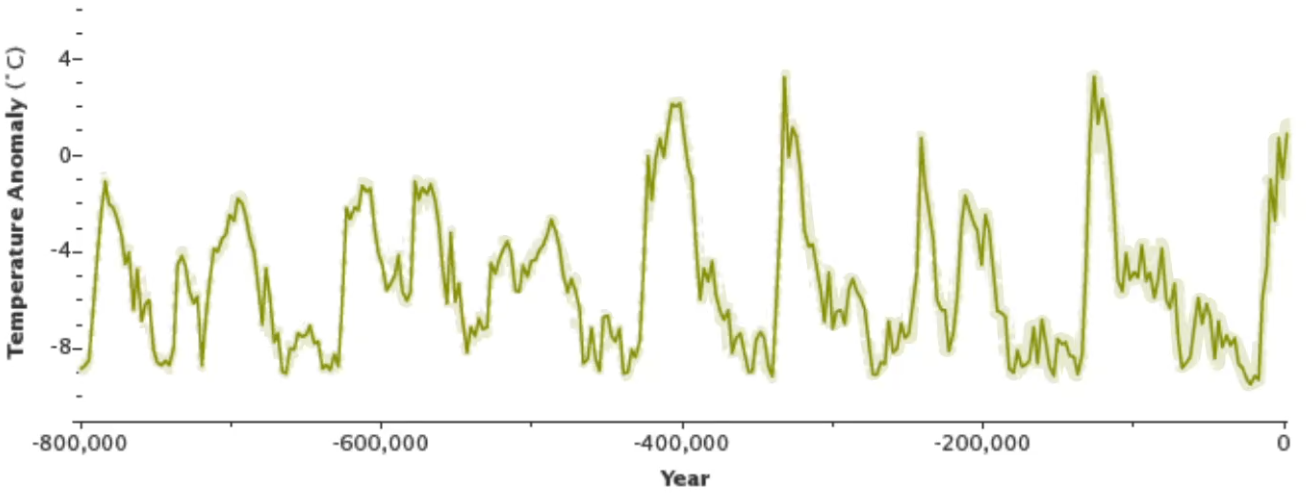
\includegraphics[width=0.7\linewidth]{../images/1-antarctic-ice-records.png}
					\caption{Antarctic ice records}
					\label{fig:1-antarctic-ice-records}
				\end{figure}
			
			\subsubsection{Causes of climate change}
				There are a few factors which cause the change in climate on earth:
				\begin{itemize}
					\item Variations in the earth's orbit around the sun (eccentricity)
					\item The axis of the Earth from pole to pole is tilted compared to this plane of movements, this is time dependent (obliquity)
					\item Precession of the Earth. 
				\end{itemize}
				Of these especially obliquity is important. It can lead to very hot summers and very cold winters without a lot of snowfall. This leads to a shrinkage in the ice coverage of the Earth which leads to ever warmer temperatures. This feedback loop amplifies itself (albedo feedback). Another factor is the physical place of land mass. If it is close to the poles, ice can easily form and reflect heat back into space. Volcanic explosions are known to have an influence as well due to their tendency to throw light blocking particles in the atmosphere. Lastly the activity of the sun itself plays a role in the climate of the earth. \\
				\\
				Us humans have had an impact since the industrial revolution by throwing tiny particles in the air due to burning fossil fuels, cooling the earth. This effect is overshadowed by the fact that we emit a lot of greenhouse gasses whilst we burn the same fossil fuels. An illustration of our impact on $CO_2$ levels can be seen in figure \ref{fig:1-co2-history}.
				\begin{figure}[h]
					\centering
					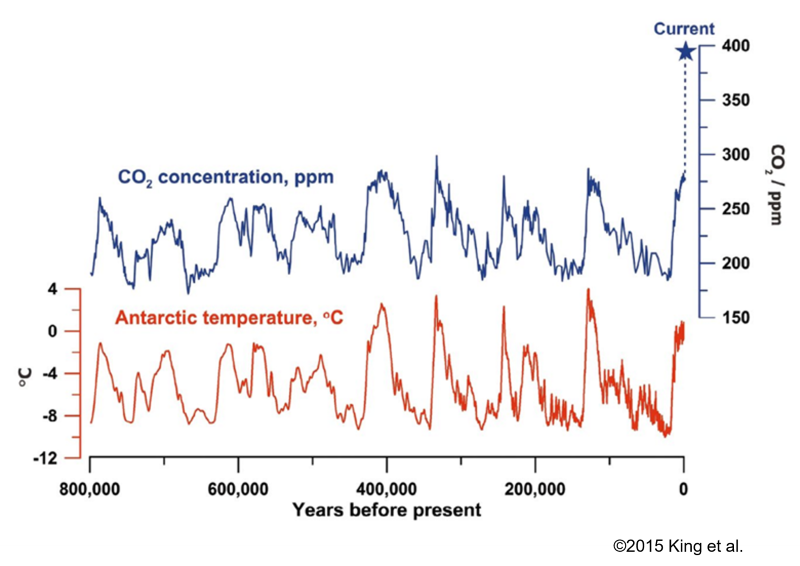
\includegraphics[width=0.7\linewidth]{../images/1-co2-history.png}
					\caption{Historic $CO_2$ records}
					\label{fig:1-co2-history}
				\end{figure}
				
			\newpage
			\subsubsection{Human cause}
				Global temperatures have increased by 1.1 degrees Celsius since industrialization. There are five lines of evidence that our greenhouse gas emission is responsible for this:
				\begin{enumerate}
					\item We see that our activities with fossil fuel and cement produces about 9Gt of carbon per year, whilst the natural rate is only 0.9Gt per year. Luckily for us, the earth absorbs about 5.5Gt per year back into itself, otherwise $CO_2$ levels would be double of what they are right now. 
					\item We also look at the isotopic ratio between C13 and C12 carbon. The gradual lowering of this ratio suggests a lot of plant derived carbon sources (fossil fuels) have been dumped in the atmosphere. 
					\item The physical mechanism by which greenhouse gasses prevent infra-red radiation from escaping our atmosphere has been proved already in 1850.
					\item Climate models where factors can be individually adjusted also show a large effect of our activity.
					\item Radiative forcing is what happens when the amount of energy that enters the Earth's atmosphere is different from what leaves it. This, again, is influenced by greenhouse gasses.
				\end{enumerate}
			
			\subsubsection{Radiative forcing}
				As discussed in the previous section, radiative forcing has an impact on our climate, but how does it work? The only way in which the earth can exchange energy is through radiation interactions with space. This is depicted in figure \ref{fig:1-radiation-exchange}.  In the end, about 31\% of the solar radiation is reflected. This yields a net solar radiation of about 235 watts per square meter. In reality this net radiation is counteracted by the natural infra-red radiation of earth, balancing the entire system. \\
				\\
				By emitting too many greenhouse gasses, we have brought this balance to an end, resulting in a net increase of energy. To investigate the forcing effect we have, we can look at a concept called radiative forcing. This is a very important concept in the whole climate research and also very important for policy implications because with this metric, we can estimate the effect of different forcing factors.\\
				
				\begin{figure}[h]
					\centering
					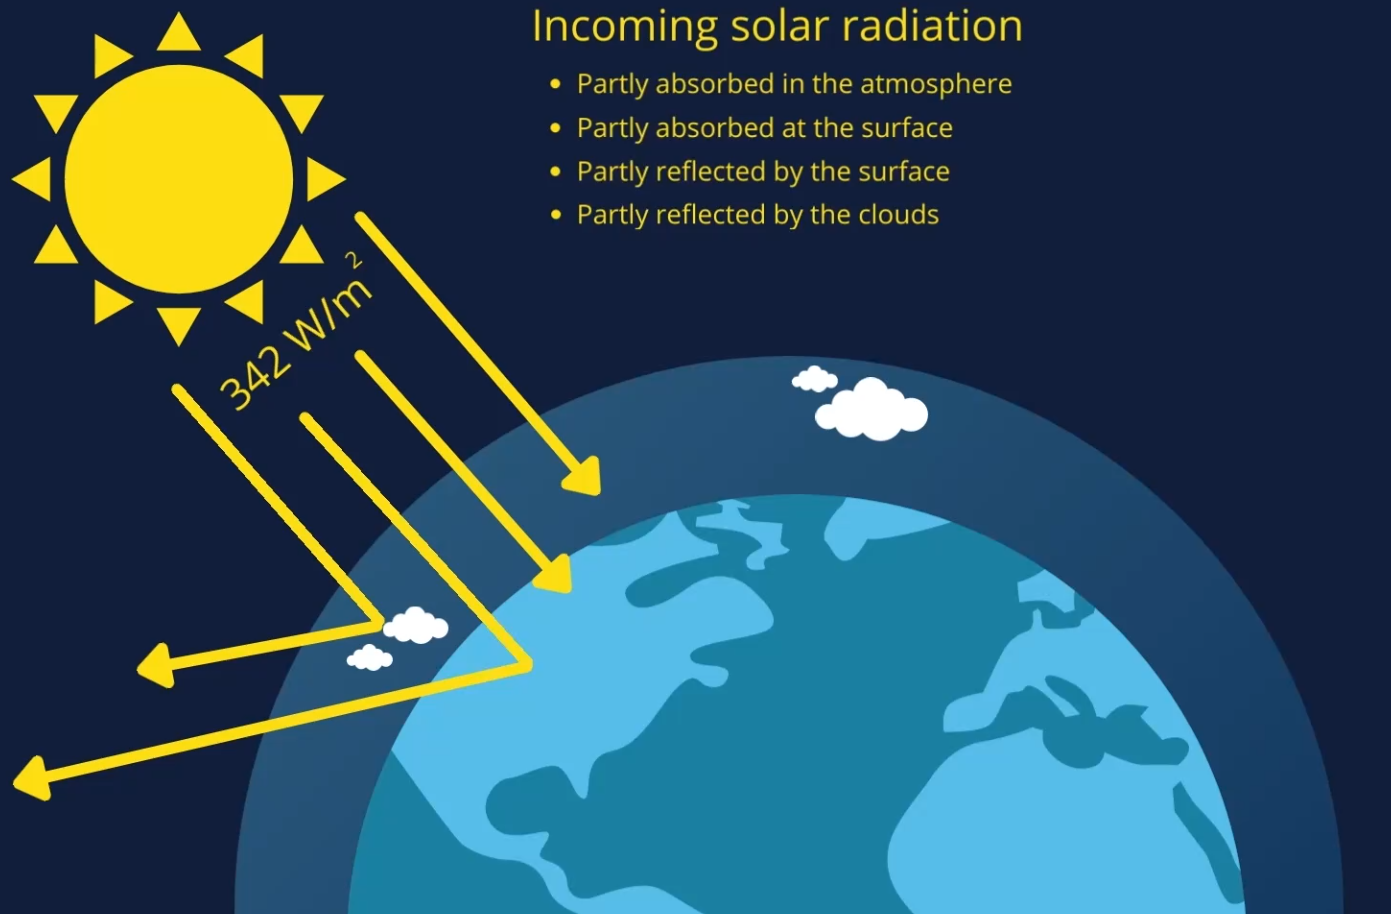
\includegraphics[width=0.7\linewidth]{../images/1-radiation-exchange.png}
					\caption{Earth's radiation exchange}
					\label{fig:1-radiation-exchange}
				\end{figure}
				\newpage
				So when we sum everything up over the time period 1750 till now, then we can also look at the average radiative forcing over that time period. The radiative forcing by carbon dioxide is the largest contributor - so that's why we talk about CO2 a lot when we are talking about climate change - namely 2.16 watts per square meter. Other well-mixed gasses also play an important role, so they also cause a positive radiative forcing. Ozone as well.
		\subsection{Climate targets and pathways}
		
		\subsection{Climate mitigation}
		
		\subsection{What can we expect for the future}
	
\end{document}